\chapter{综合语义修复与实际 FPGA 实验}
\label{ch:synthesis-repair}
本章区分三类实验：用于定位错误的失效网表、通过独立功能见证的小单元网表，以及完整顶层的综合和实现。它们采用的 DUT 尺寸、通过判据和可推论范围不同，不能合并成一个笼统的“Vivado PASS”。所有原始失败工件保留；最终评审状态通过额外记录说明，不覆盖历史 manifest。

\section{为什么原先的综合数字必须作废}
第一次完整顶层综合虽然生成了利用率和时序报告，日志却出现五条无驱动诊断，
编号均为\code{Synth 8-3848}。
其中包括 \code{sadc_enc} 的树根计数，以及 \code{cal_weight_reduce} 的根归约量。
旧写法把节点信号定义在每个 generate 作用域中，再以
\code{g_node[2*t].total} 等前向层级名称连接子节点。
在本次 Vivado 2018.3 实跑中，这些根节点的驱动关系未被正确保留。
同一源码在 Verilator 中能正确求值，说明只用一个 RTL 仿真器不足以发现该类映射差异。

随后读取 DCP 内的网表，发现基线的 Flash 输入仅保留端口声明，没有通向逻辑的实际扇出；
归约模块则丢失了正常输入和加权树。进一步的小单元网表仿真在第一个 Flash 检查就观察到高阻态 Z，
而独立参考值为零。这是功能不一致的直接证据。
因此，原来的 35,902 LUT、65,454 FF 与 $-15.874$\,ns WNS 只保留为故障诊断数据；
同类旧列共享快照的 35,806 LUT、65,370 FF 与 $-16.228$\,ns WNS 也不属于有效 PPA 比较。
资源数很小有时意味着逻辑被错误删除，不能先把它解释为优化收益。

\section{修复的结构原则}
修复后，树边信号在模块作用域显式声明，generate 只负责给确定索引的节点赋值。
每个有效节点仍满足
\begin{equation}
Y_t=Y_{2t}+Y_{2t+1},\qquad 1\le t<L,
\end{equation}
叶子与补零规则不变，根输出仍为 \(Y_1\)。
这里 \(L\) 为覆盖有效叶子数的二次幂。
改写没有把平衡树变成一个顺序累加环，也没有增加寄存器或改变结果延迟。
所有节点有唯一驱动；padding、单叶几何和最大支持几何都必须能展开。

旧版之所以选择命名节点，是为了避免某些 lint 工具把聚合数组误判为循环。
新实现对 Verilator 使用 \code{split_var} 注释，指明常量索引元素可以分开分析；
该注释不是屏蔽 \code{UNOPTFLAT} 之类的诊断，也不会改变 Vivado 的逻辑方程。
严格 lint 继续作为失败门禁。两种工具对写法的可接受性都纳入验证后，才算解决了工程兼容性问题。

\section{同一刺激下的 RTL 与网表对照}
独立见证模块同时包含 3-bit 和 9-bit Flash 编码器，以及 3 个物理 slice、每个 2 主加 1 子单元的归约器。
它有 969 个输入位，使用 48-bit 系数、64-bit 总和和 66-bit 带符号轨和。
这是一种为快速映射检查选定的小尺寸，不是 18\(\times\)71 生产几何的替代。

参考算法逐个物理单元累加，既不遍历 DUT 的树，也不调用 DUT 的借位或归约辅助函数。
12,904 个默认检查由五组构成：128 个 3-bit 编码器输入位型、512 个 9-bit 温度计状态、
3072 个合法两-slice 选择与开关/模式组合、8192 个全部地址编码与轨模式组合，
以及 1000 个全 48-bit 系数和非温度计 Flash 位型的伪随机组合。
相同 testbench 分别驱动原始 RTL 和 Vivado 导出的功能网表。

\begin{table}[H]\centering\small
\begin{tabularx}{\textwidth}{p{36mm}X X X}\toprule
版本&RTL 语义检查&网表输入因果&XSim 功能检查\\\midrule
旧前向引用写法&12,904 次通过&959/969 个输入无端点扇出&首个 Flash 检查失败，得到 Z\\
旧公式，仅修树连线&12,904 次通过&969/969 个输入有端点扇出&12,904 次通过\\
列共享公式，修树连线&12,904 次通过&969/969 个输入有端点扇出&12,904 次通过\\
\bottomrule\end{tabularx}
\caption{相同独立见证下的真实对照。扇出恢复是必要条件；逐值检查进一步检验函数，二者不能互相替代。}
\end{table}

小单元映射的旧公式连接修复版为 2834 LUT，列共享修复版为 1837 LUT，两者均为纯组合见证，
FF 和 DSP 为零。该实验说明列共享在这个具体尺寸和工具设置中有资源收益，
但不能把减少的 997 LUT 或局部比例外推到包含系数存储、MAC、调度和除法器的完整 ADC 数字顶层。
错误旧版只剩 2 LUT，明确排除在收益计算之外。

\IfFileExists{figures/38_tree_mapping_trace.png}{
\begin{figure}[H]\centering
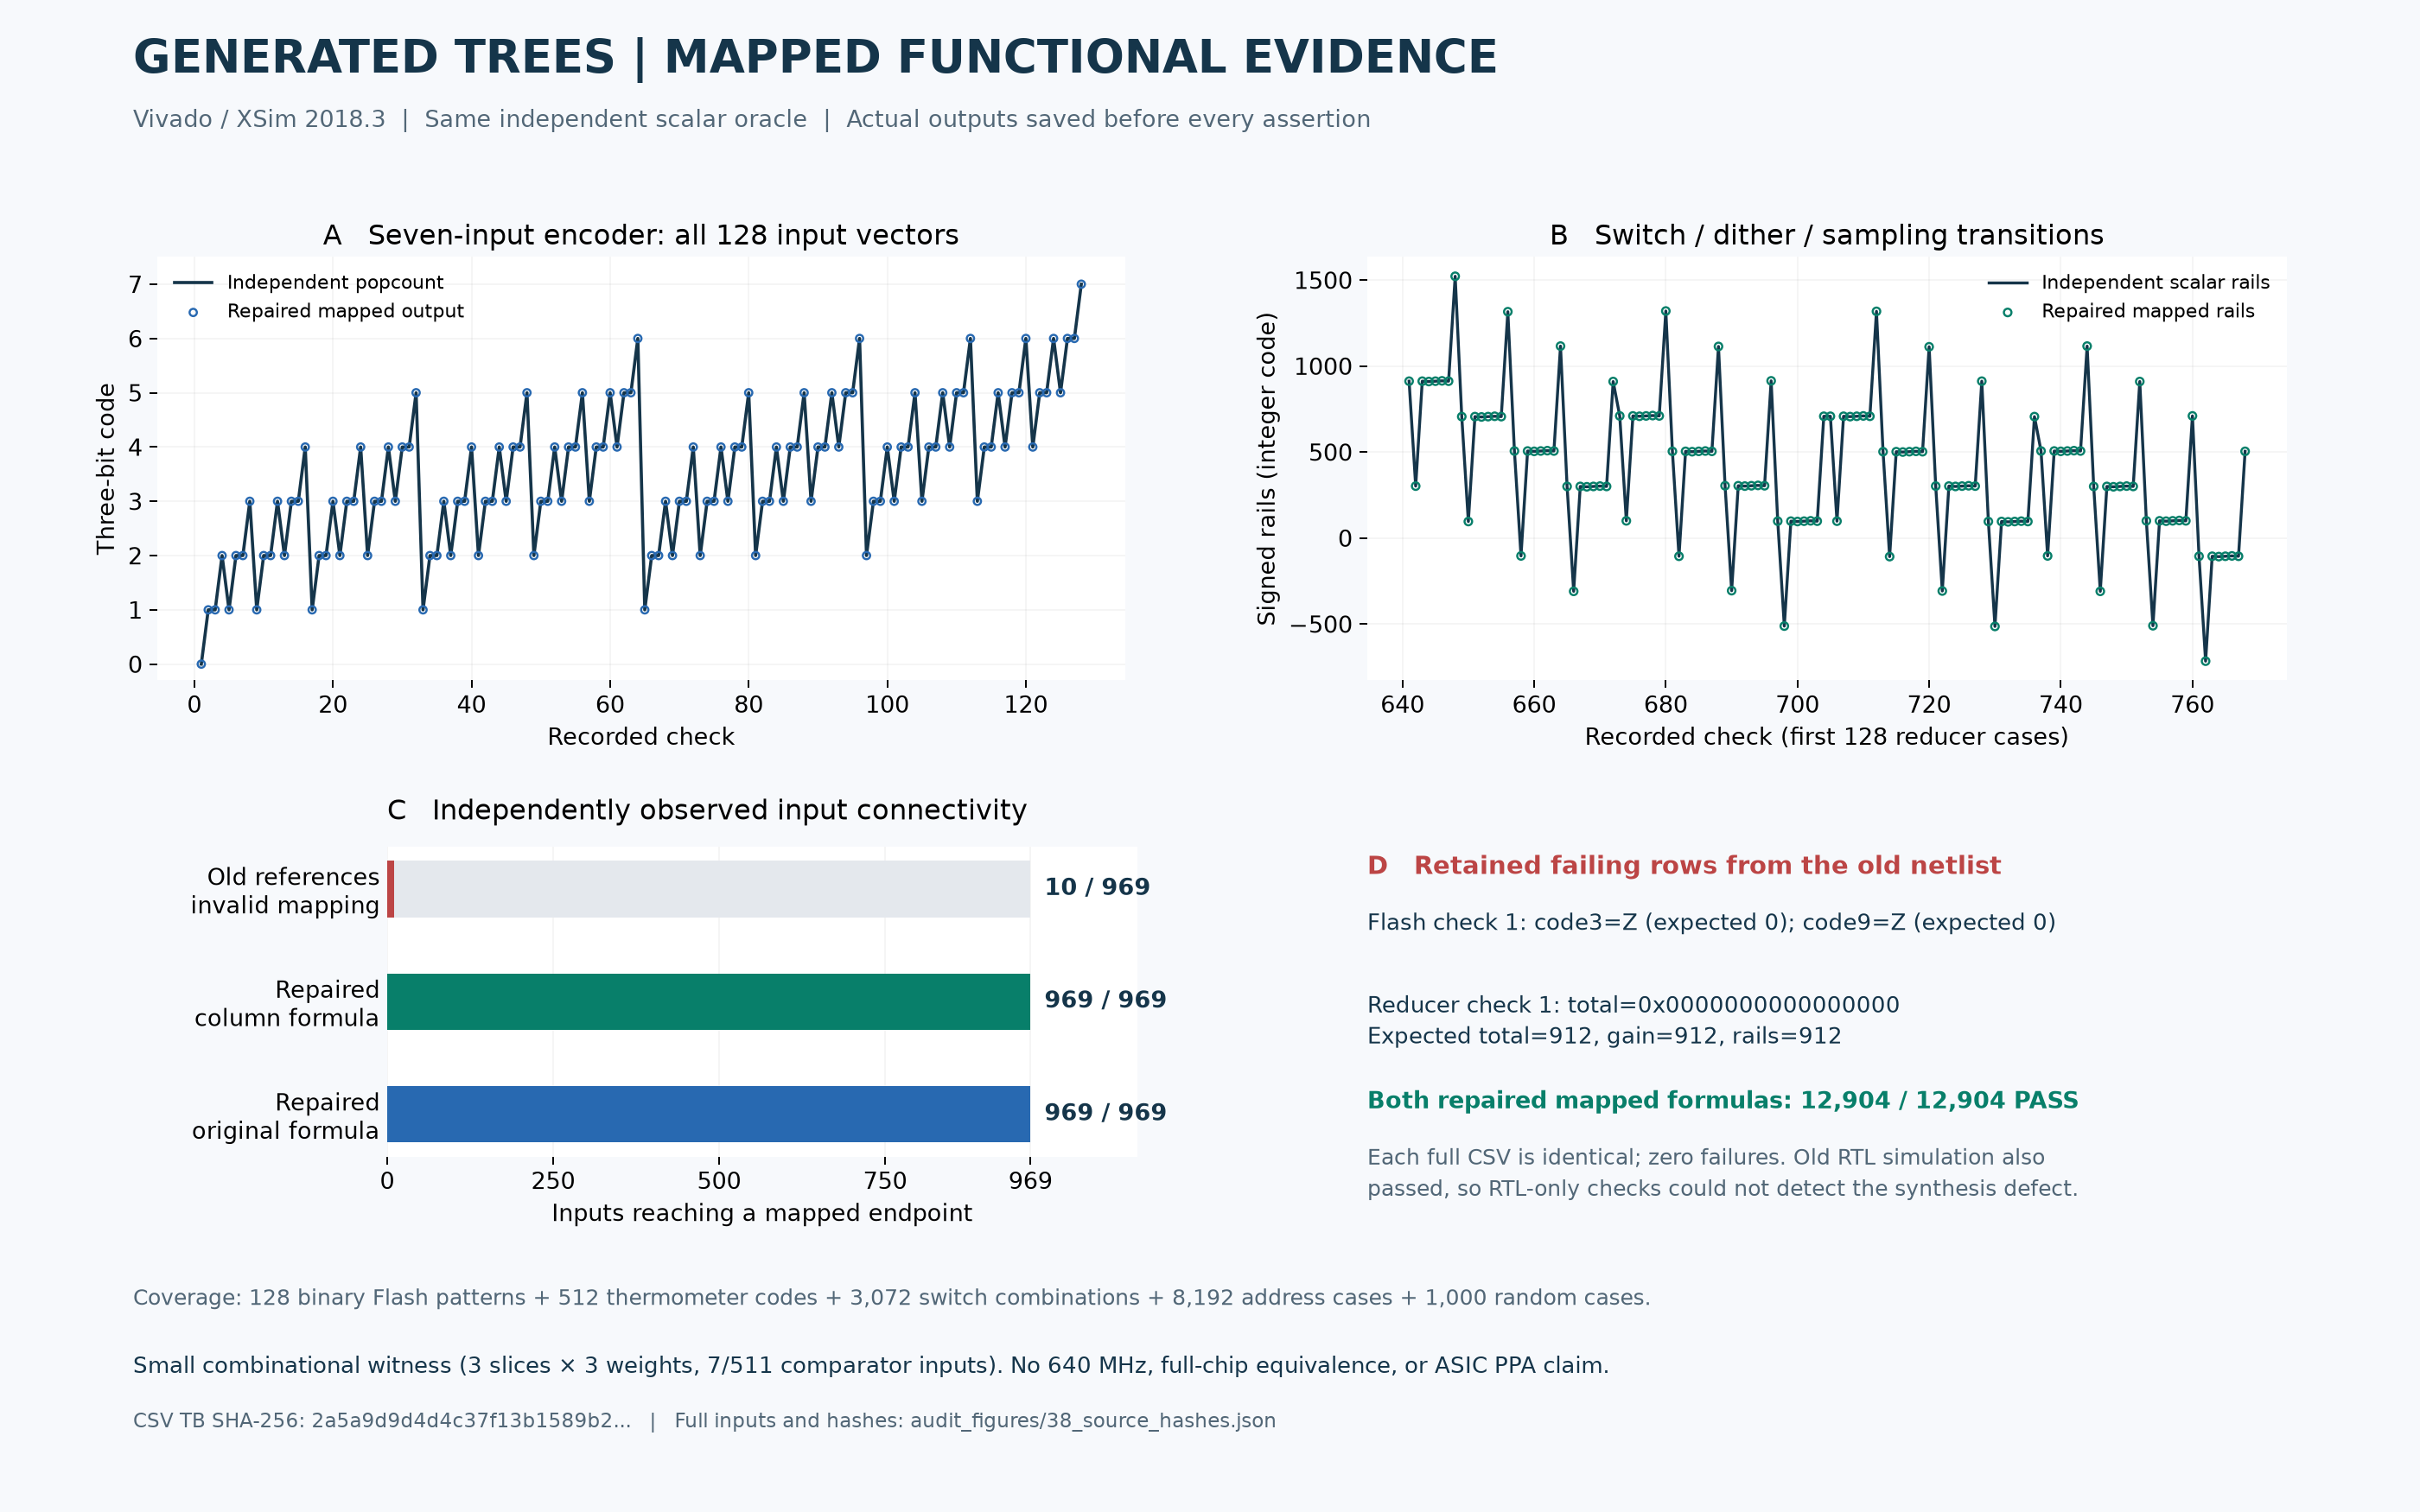
\includegraphics[width=\textwidth]{figures/38_tree_mapping_trace.png}
\caption{映射见证的实际输出、期望值和故障行。图由原始 XSim CSV 及输入扇出记录生成；高阻/未知值作为错误保留，不转换为数值零。}
\end{figure}
}{}

\section{完整顶层的公平对比条件}
新完整基线和优化版均先修复树连线与 Flash 编码器的映射问题。
基线保留列共享之前的归约公式和原除法实现；优化版包含列共享与借位复用两项算术优化。
因此，完整顶层前后差异属于这两项优化的组合效果；若要分别归因，还需要增加仅改变其中一项的实验。
两份隔离快照保留所有文件 SHA，其他生产 RTL、器件、工具和脚本保持一致。
后续精简 P5 配置还包含权重恒零最高位的显式掩蔽。
因此，P7 基线对 P7 列共享/借位版是第一组公平 A/B；
该 P7 版对精简 P5 版则同时改变除法展开参数、权重存储表达式和周期约束（P5为25\,ns），
属于整体配置比较，不能把全部差值单独归因于 P5 参数，也不能称为同约束面积对照。

器件为 \code{xc7vx690tffg1761-2}，Vivado 版本为 2018.3，综合顶层为
\code{sar20_digital_core}，结构模式开启，保留全部可写物理权重。
采用 \code{out_of_context} 与 \code{flatten_hierarchy=rebuilt}，线程数为 2。
申请周期 1.5625\,ns 在该版本的时间网格上成为 1.563\,ns；报告同时保留申请值与实际值。
0.05\,ns 用户时钟不确定性和零 I/O delay 是结构筛选条件，不能据此假定真实比较器或板级接口无需建立时间。

P5/P6/P7 的 RTL 协议回归都保持 16 拍输入间隔，输出延迟分别为 15/13/11 拍。
综合配置的比较还需考虑关键路径是否从除法转移到权重归约或 MAC。
将一条路径缩短后，新的最坏路径可能来自另一模块；这是优先级转移，而不是测量矛盾。
不应只摘取 \code{u_div} 的改善值来宣称顶层频率提高。

\IfFileExists{sections/vivado_measured_table.tex}{\subsection{P7 公平 A/B 的实际结果：面积退化而非收益}
\begin{table}[H]\centering\small
\begin{tabular}{lrrr}\toprule
指标&修复后基线 P7&列共享/借位 P7&变化\\\midrule
Slice LUT&171,246&199,039&+27,793（+16.23\%）\\
FF&66,817&66,778&$-39$\\
DSP48&20&20&0\\
BRAM / latch&0 / 0&0 / 0&0\\
Setup WNS（ns）&$-17.426$&$-17.112$&+0.314\\
Hold WHS（ns）&$-0.264$&$-0.264$&0\\
Pulse width slack（ns）&+0.025&+0.025&0\\
最坏数据路径（ns）&18.941&18.627&$-0.314$\\
最坏路径逻辑级数&135&148&+13\\
该路径 CARRY4 数&117&125&+8\\
Vectorless 估计（W）&1.58&1.58&报告精度内相同\\\bottomrule
\end{tabular}
\caption{相同器件、Vivado 2018.3、P7 与申请周期1.5625\,ns的完整综合结果。均为综合后估计，尚未布局布线；功耗未使用实测开关活动。}
\end{table}

这组结果否定了“源码加法表达式变少就必然节省 FPGA 面积”的假设。
列共享与借位改写的组合使 LUT 增加16.23\%，setup只改善0.314\,ns，仍大幅违反目标。
最坏路径仍位于除法器：基线从\code{dv_reg[0]}到\code{q_reg[60]}，
改写版从\code{rem_reg[0]}到同一目标寄存器。
改写后125个CARRY4串联，说明每拍展开7步的串行借位依赖仍是主要频率障碍；
FF仅减少39个，不足以抵消组合资源增长。
因此，这一版本只能称为功能等价的算术结构候选，不能宣传已经获得低面积PPA优势。

两份\code{check_timing}的16类问题计数均为0，未约束路径表为空；
这说明记录约束下的检查覆盖，并不消除实际负setup/hold裕量。
OOC时钟尚未通过真实内部BUFG布线，且I/O延迟为零，
所以不能从18.627\,ns的综合估计直接宣布53.7\,MHz为可用频率。
后续P5以25\,ns进行FPGA筛选，另外改变了展开数、权重最高位表达式和时钟约束；
必须单列其结果。行和缓存若进入候选，也须与该P5在相同25\,ns条件下比较。

基线DCP为69,108,593字节，摘要\code{9c3bc09dd193d0bf}\ldots；
列共享/借位DCP为71,421,073字节，摘要\code{4712577f4291fed3}\ldots。
两份均已逐字节核对远端与本地SHA-256；原始报告、源归档和完整摘要见
\code{docs/evidence/20260930/vivado_complete_p7/}。
第一份运行曾在报告下载阶段超时，原失败manifest保留，随后从同一次已完成运行恢复并验证；
不能把文件传输故障混写为综合失败，也不能只凭恢复状态略去原始过程。
}{}
\IfFileExists{figures/32_vivado_comparison.png}{
\begin{figure}[H]\centering
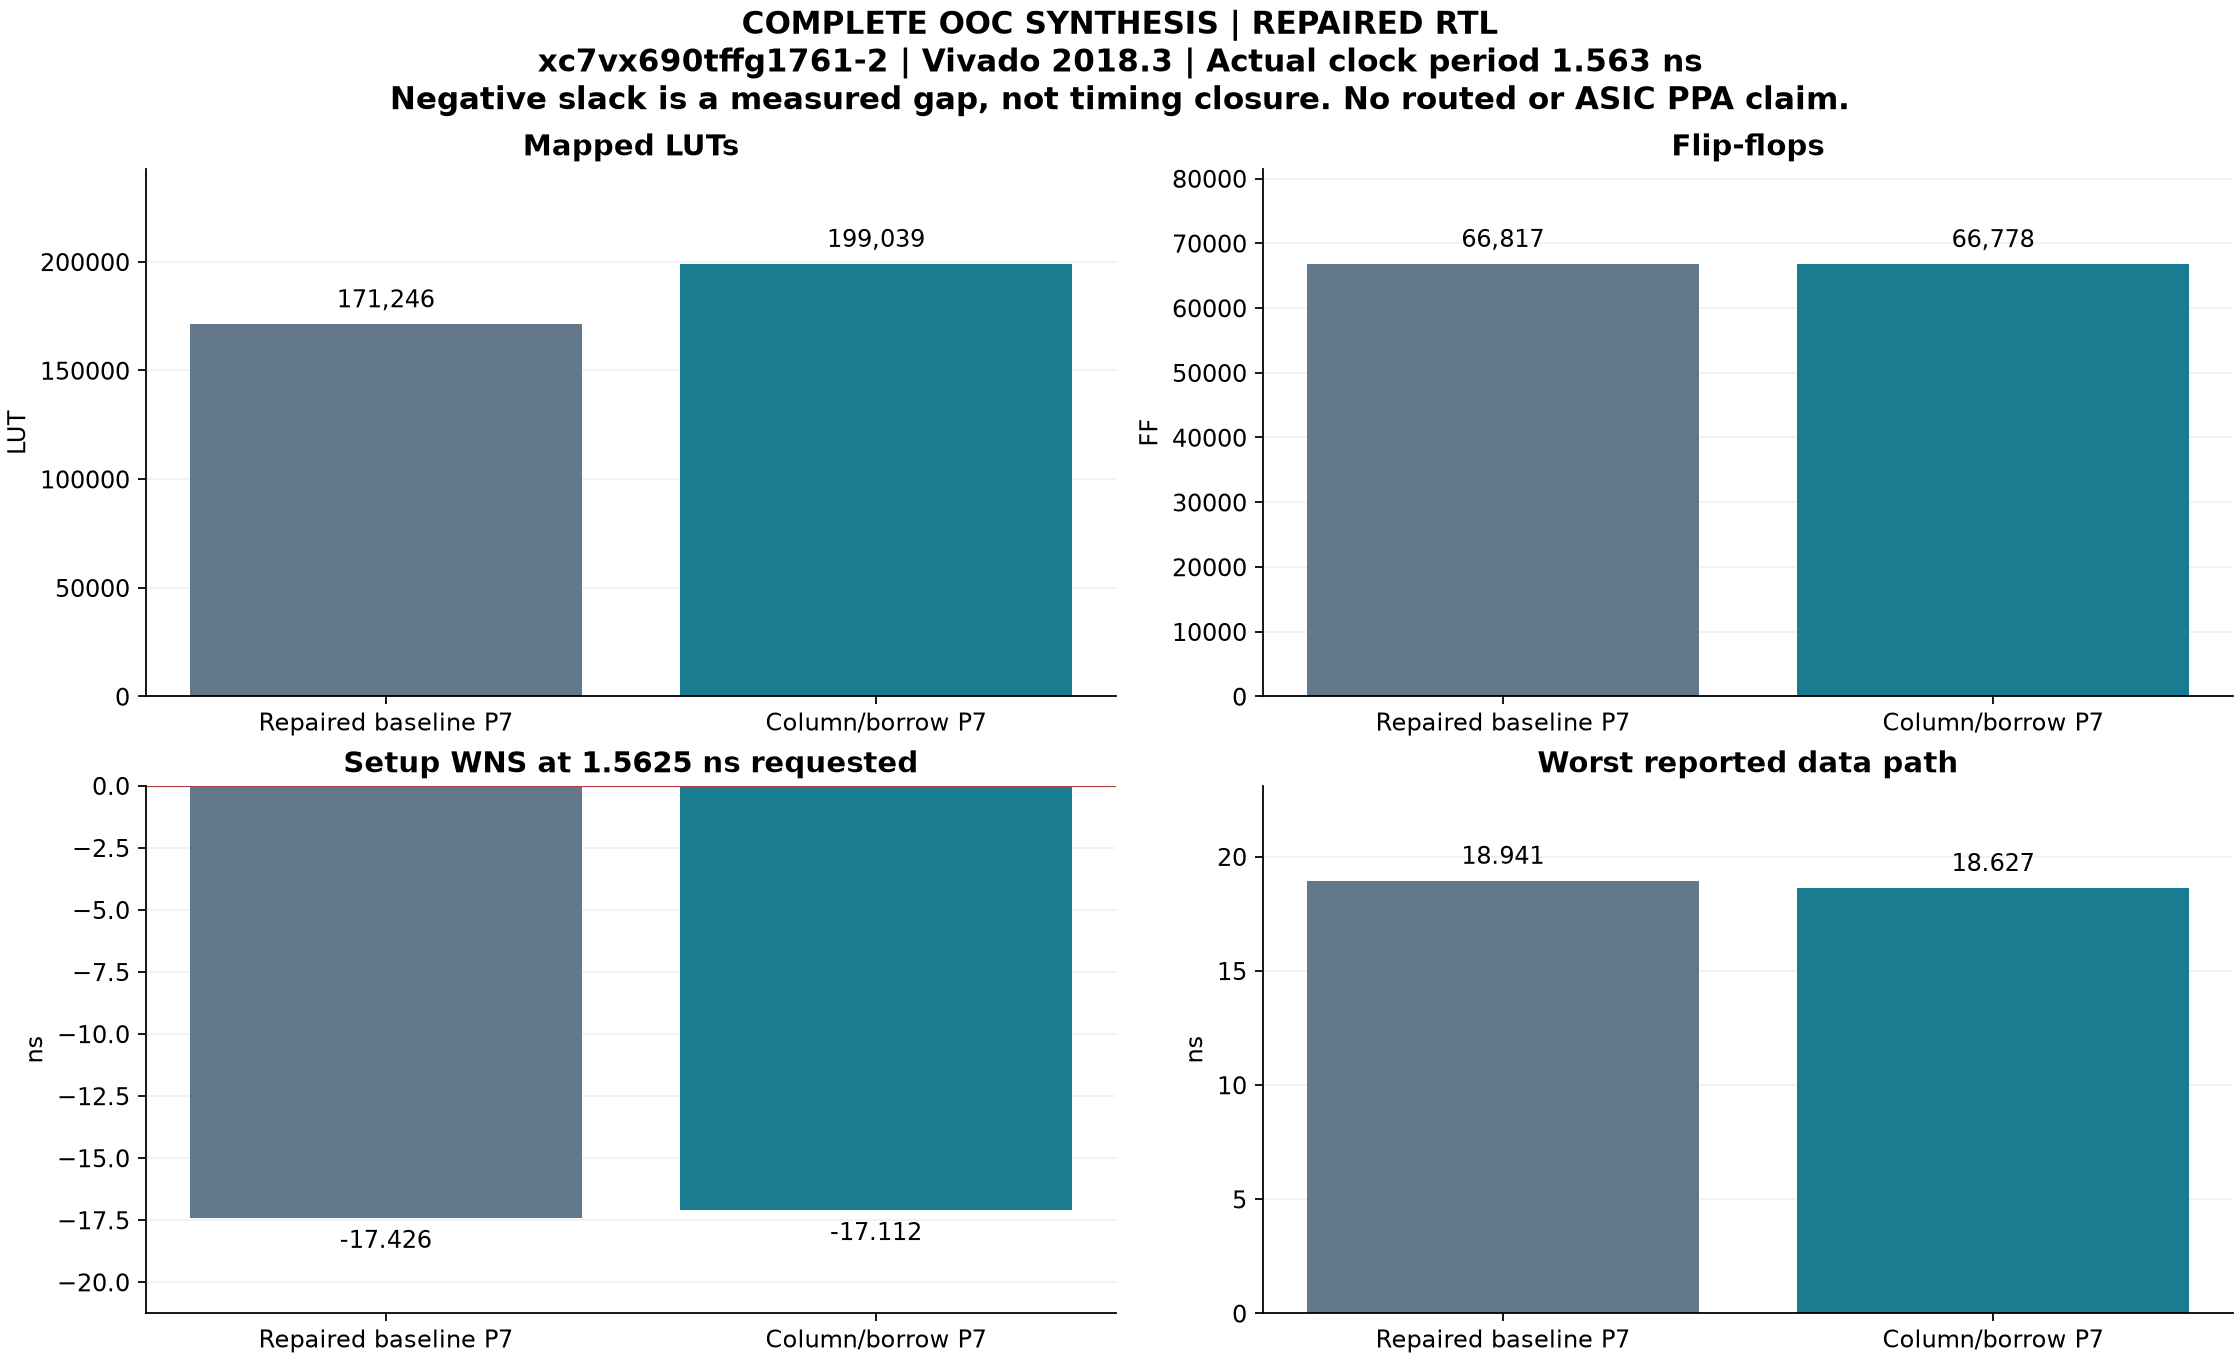
\includegraphics[width=\textwidth]{figures/32_vivado_comparison.png}
\caption{有效完整顶层快照在相同 FPGA、工具和申请周期下的综合后对照。负 WNS 表示与该目标的差距；该图不表示布线后或 ASIC 时序闭合。}
\end{figure}
}{}


\section{资源开销的解释与进一步缩减条件}
有效完整基线的 \code{weight_store} 实测为 62,622 FF，
恰好等于 \(18\times71\times(48+1)\)：每项 48-bit 系数加一位本 epoch 已写标记。
它约占该基线全部 66,817 FF 的 93.7\%。
因此，单纯把除法余数寄存器缩窄几位，无法解决主要寄存器开销。
这个数字也说明，当前“全部物理权重可同时读取”的接口具有实在的面积成本。
必须把这种成本与论文未披露的实际系数存储结构区分开。

这里还能提取一个可综合的不变量。合法写入必须满足 \(0<W<2^{47}\)，
复位将权重置零，clear 只清除已写标记，拒绝写入保持原值。
因此，从复位状态开始逐拍归纳可得所有物理权重的 bit 47 恒为零。
基线 DCP 仍存在 1278 个名为 \code{w_q_reg[s][u][47]} 的 FDRE，
表明综合器没有利用跨越写入许可逻辑的这一数值关系。
本轮后续精简版将接受写入时的存储表达式显式写为
\begin{equation}
W_{\rm stored}=W_{\rm data}\mathbin{\&}(W_{\max}-1),\qquad W_{\max}=2^{47}.
\end{equation}
对任何被接受的写入，该表达式逐位等于原始数据；原 48-bit 端口和非法写入拒绝条件不变。
这属于把已经成立的常量位显式暴露给综合器，不是降低合法系数精度。
实际删除数量仍以该精简版 DCP 和资源表为准，不能仅按预计数填入测量栏。
\begin{figure}[htbp]
  \centering
  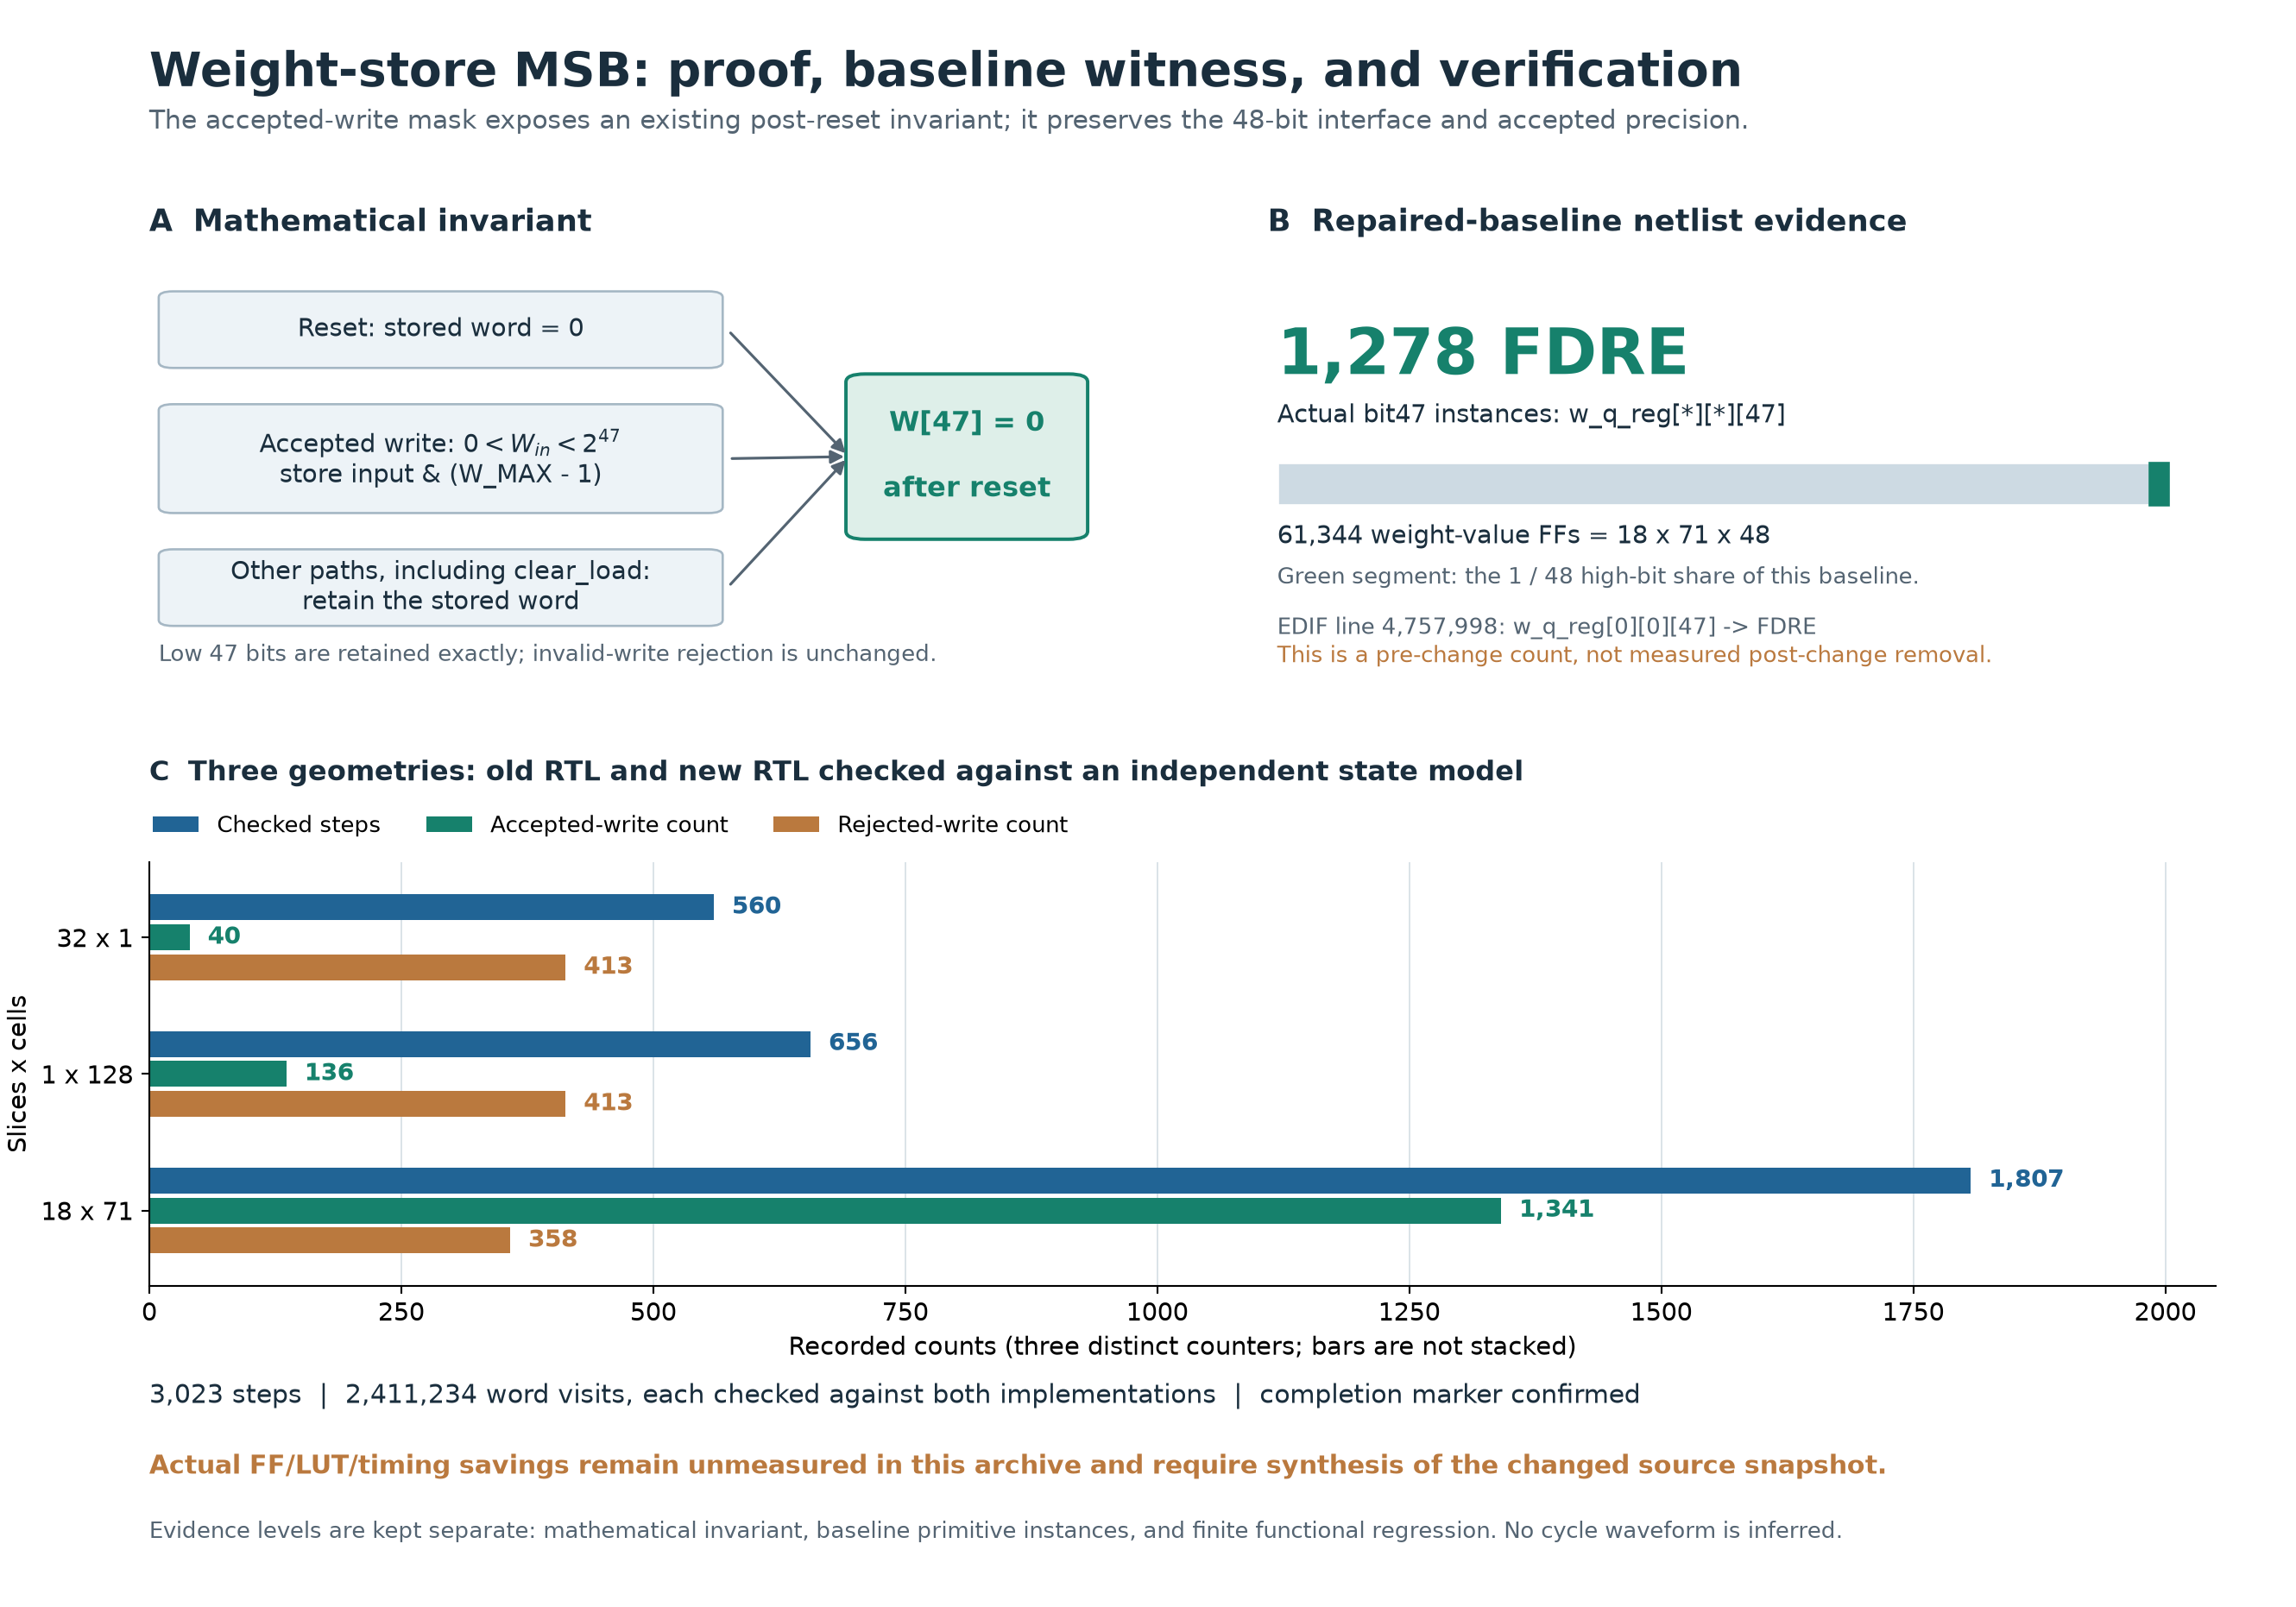
\includegraphics[width=\textwidth]{figures/40_weight_msb_evidence.png}
  \caption{权重存储最高位优化的三层证据。A：复位写零、合法写入满足$0<W<2^{47}$、其他分支保持原值，因而可由归纳法证明复位后的$W[47]=0$；显式写入掩码保留低47位及原有非法写入拒绝行为。B：修复后的基线网表中，61,344个权重数值触发器确实包含1,278个第47位FDRE实例，绿色段仅表示这一基线的$1/48$份额，不能解释为已测得的优化后面积节省。C：三种几何配置的独立状态参考分别检查560、656、1,807步，共3,023步；接受写入、拒绝写入与检查步数是三个不同计数器，图中不堆叠、不相加。按各配置的检查步数乘以存储单元数，共访问2,411,234个权重字，每次均对照修改前、修改后实现；不能再将两种实现的比较次数倍增为覆盖数量。数据来自\code{weight_msb/verification_manifest.json}、\code{equiv.run.log}与\code{vivado_structure/baseline_weight_msb_witness.json}，制图脚本逐项核对归档哈希与完成标记。图中没有重建逐拍波形；修改后真实FF、LUT和时序收益仍需对相应源码快照重新综合测量。}
  \label{fig:weight-msb-evidence}
\end{figure}


综合报告没有推断出 BRAM。若改为块 RAM，必须同时设计读端口数、系数供给带宽、
样本上下文流水与 epoch 清空协议，不能只把数组声明换一个关键字。
每笔 8 个活动 slice、每个 71 个权重，若完全逐项读取则每笔至少需要 568 次系数访问。
16 拍启动间隔意味着平均至少 35.5 项每拍；这是访存下界，尚未计入配置读回和装载。
即使总带宽足够，每个活动物理 slice 都需要在窗口内供出自身 71 项，
所以按 slice 分 bank 的双端口 RAM 还会遇到每 bank 的独立带宽限制。
增加复制读端口、预存前缀和或装载期预聚合，都需要新的面积、同步和数值等价测量。

另一个无需增加寄存器的组合候选是利用同一物理行的共享选择条件：
\begin{equation}
T=\sum_s A_s\!\left(\sum_u W_{s,u}\right),\qquad A_s\in\{0,1\}.
\end{equation}
它把逐权重选择改为逐行总和选择；开关项若能证明 \(on_{s,u}=1\Rightarrow A_s=1\)，
也可以消去重复的活动行门控。
但生产几何下，简单二级平衡树可能形成 \(7+5=12\) 层，原全局树为 11 层。
活动行控制到输出可能缩短，而系数寄存器到输出可能增长；因此必须分别测量两类路径，
不能只数门控数量便断言时序改善。这一候选尚未计入本轮资源收益。

静态 \(T\) 与部分模式相关 \(G\) 可以候选地在配置装载期累计，
但当前结果依赖物理 slice 组合、采样 dither 掩码和 DEM 后的物理开关。
对 \(R\) 的优化必须保留真实 \(on\) 与轨极性，不能把物理失配权重退化为均匀权重或名义码乘常数。
一种可检查的推进顺序是：先缓存每个 slice 的总和与专用采样单元和，
再将未加权的选择状态同缓存版本一起锁定到 epoch；
最后以现有逐物理单元 oracle 对最大系数、所有模式、重复地址及 clear 中断逐值核对。
上述方案中的每行总和缓存已在后文实现并做定向验证；专用采样单元和缓存、额外流水及存储bank仍为候选。功能验证通过不等于面积改善，行和缓存的资源收益须以独立同约束综合对照为准。

还需注意 \code{flatten_hierarchy=rebuilt} 的资源归属。
Vivado 会在扁平优化后重建层级，逻辑可以跨原始 RTL 边界移动；
例如有效基线重建的 \code{cal_sample_context} 接口包含原 RTL 没有的归约相关端口。
因此，“该层级下 LUT 很多”不能直接推成“打包上下文寄存器产生了这些 LUT”。
顶层利用率才是整体 A/B 比较的直接计数；模块优化的归因还需要保留边界的独立综合、
原始 primitive 连接与功能检查，不能只根据重建层级名称修改 RTL。

\section{可实现频率与布局布线验收}
用户确认的验收口径允许 FPGA 使用实测可实现频率，并保留 ASIC 640\,MHz 目标。
实现流程读取已验证和冻结的 DCP，不覆盖原综合结果；在新输出目录设置明确周期，
依次运行 \code{opt_design}、\code{place_design}、\code{phys_opt_design} 和 \code{route_design}。
setup、hold、脉宽、路由完整性和 DRC Error 分别检查，不能只按 setup WNS 生成成功标记。

原始外部时钟筛选流程通过 \code{HD.CLK_SRC} 指定实际存在的 BUFGCTRL site。
AMD/Xilinx 文档明确指出：当缓冲器位于 OOC 模块之外时，该全局时钟不在模块实现中实际布线；
该属性提供驱动位置/类型以改进时钟延迟、偏斜与共同路径悲观移除估计。
因此，本次进一步准备了带内部 BUFG 的实现流程：仅断开顶层 \code{clk} 端口与原时钟网的直接连接，
将端口接至 BUFG 输入，再以其输出驱动原来的完整时钟负载集合。
ECO 前后所有时钟端点的排序列表、数量与 SHA-256 必须相同；只允许增加一个 BUFG，
不能因引入时钟缓冲而删改数据通路或丢失寄存器。

实现后另检查 BUFG 输出网的实际 \code{ROUTE_STATUS=ROUTED}、非空 routing nodes/pips，
并分别读取全设计与内部寄存器路径的 setup/hold 最坏裕量。
还要求脉宽裕量非负，TNS/THS/TPWS 与三类失败端点数均为零；
\code{check_timing} 的16项覆盖计数必须齐全且全部为零，未约束与忽略路径分组必须为空。
报告缺失、字段不全、非有限数或摘要与逐路径查询不一致均不能产生通过结论。
这只说明记录下来的 OOC 约束被完整检查，不证明零 I/O 延迟适合真实板级接口。
\code{HD.CLK_SRC} 的估计上下文不再代替内部时钟布线。
该流程依然是 OOC：端口至 BUFG 输入的外部时钟边界及零 I/O delay 不是整板接口约束。
所以内部时钟实际布线与整板时钟签核必须分别表述；本流程不输出整板 bitstream 验收，
也不替代 ASIC PVT 与物理库签核。
参见 \href{https://docs.amd.com/api/khub/documents/dUZkF9u9qQ4x4MtRgpH9aQ/content}{UG905 v2018.3}。
109 个缓冲时钟流程与报告解析用例已通过；六组流程合计272项通过。
这些是前置工程验证；只有后面的实际运行表能证明布局布线结果。

Vivado runner 的 Windows 外层批处理可能在 Tcl 负时序退出后仍返回 raw 0。
流程保留原始返回码，只在完整状态文件、参数、工具版本、全部所需报告和负 WNS 一致时，
才把它解释为“综合完成、时序未满足”。任何无驱动告警则使综合完整性失败，
不能再把该网表放入有效 PPA 对照。用于控制这种行为的 mocked tests 验证流程逻辑，
真实综合/实现报告验证 EDA 的实际结果，两者分开计数。

\section{配置期行和缓存：把不随样本变化的加法移出转换路径}
\label{sec:row-cache}
P7 实测的 LUT 退化促使本轮重新选择优化对象。对于同一个生效配置 epoch，
物理系数不变，只有活跃 slice 集合与开关状态变化。因此可以把
\(H_s=\sum_u W_{s,u}\) 缓存在系数装载器中，转换时只计算
\begin{equation}
T=\sum_s A_s H_s,\qquad
G=T-M,\qquad R=T-2W_{on}+R_d.
\end{equation}
其中 \(A_s\) 是物理行是否活跃的位图，\(M\) 和 \(R_d\) 仍按实际采样轨求和。
这不是拟合算法，也不是论文披露的新电路；它是当前可编程整数校正接口的精确工程变换。
本节描述行和缓存候选。其本地22项功能回归已完成，双版本定向与负控证据见本节末；
最终PPA取舍仍须由同约束综合及实际实现结果决定。

\begin{figure}[H]\centering
\begin{tikzpicture}[node distance=8mm and 10mm,box/.style={draw,rounded corners,align=center,minimum height=12mm,fill=blue!6},arr/.style={-{Latex[length=2mm]}}]
\node[box,minimum width=37mm] (write) {接受的配置写\\地址 $(s,u)$ 与新值};
\node[box,right=of write,minimum width=44mm] (delta) {$H_s-W_{s,u}+W_{new}$\\精确替换更新};
\node[box,right=of delta,minimum width=35mm] (cache) {18 行缓存\\每行54 bit};
\node[box,below=of write,minimum width=37mm] (store) {原物理系数表\\合法值47 bit};
\node[box,below=of cache,minimum width=35mm] (sum) {活跃位图门控\\18 行归约得到 $T$};
\draw[arr](write)--(delta);\draw[arr](delta)--(cache);
\draw[arr](write)--(store);\draw[arr](store.east)-|(delta.south);
\draw[arr](cache)--(sum);
\end{tikzpicture}
\caption{候选行和缓存的工程结构示意。系数与缓存只在同一个接受写边沿更新；这是结构说明，不是仿真波形。}
\end{figure}

\subsection{逐拍不变量与 clear 的语义}
必须证明的状态关系是每个周期都满足 \(H_s=\sum_u W_{s,u}\)，
而不是仅在完整装载结束时偶然相等。复位同时令系数和行和为零。
合法接受对 \((s,u)\) 的写入时，旧值先被减去，再加新值，系数和缓存同沿提交；
其余行不变。被拒写、运行锁定和空闲周期保持二者。
\code{clear_load} 只清除本 epoch 的 written bitmap，保留系数数值，因而也必须保留行和。
clear 之后的第一次重写仍然减去保留的旧值；若把 written=0 当成“旧系数为零”，
第二个装载 epoch 就会重复累计。这是定向负控应能识别的关键故障。

活跃行由物理 ID 的 OR 位图形成。重复 ID 会报警，但数值求和仍只包含该物理行一次；
缓存实现必须保持这一原有语义，不能改为每个逻辑槽重复累加。
无效 ID 不激活任何物理行。采样 dither 的列树继续读原物理叶子，
只移除 total 树的上层加法，不能连带删除列树仍需使用的叶值。

\subsection{宽度、资源预算和配置路径的代价}
合法写入满足 \(0<W<2^{47}\)。对一行 \(U\) 个单元，
\begin{equation}
0\leq H_s < U2^{47}\leq 2^{47+\lceil\log_2 U\rceil}.
\end{equation}
生产配置 \(U=71\) 因而需要54 bit，18行共972个候选状态位。
模块支持的最大 \(U=128\) 仍满足54 bit上界；\(U=1\) 时47 bit即可。
向原64-bit归约接口补零不会改变精度。按该上界作归纳，每次减旧值无下溢，
加新值后不越出行和宽度；此证明依赖装载器的合法写守卫，不适用于任意未经检查的外部位型。

原1278个有效叶的 total 归约需要1277次非平凡加法，
18行归约需要17次，源结构减少1260次加法。
on 树和 dither 列树保留；宽系数并行读也仍存在，不能由此宣称已转换成SRAM结构。
初版新增代价包括972个状态位、被选行和的读选择、旧系数读选择、一次减法和一次加法。
初版通过装载器的 \code{selected_weight} 显式共用写替换与配置读回的旧值路径，
避免只依赖跨层级优化来合并两个宽选择器；实际布线随后揭示这条全局反馈路径过长，
因此下面另检验逐物理行局部更新候选。

配置路径仍在同一个时钟域内，每次合法写必须满足真实 setup/hold。
不能因为软件通常慢速写寄存器，就把这条路径设为 false path 或多周期。
如果最终关键路径转移到“选择旧权重—减法—加法—行和寄存器”，
应在保留当前握手语义的前提下继续处理，或者报告实际可用频率。
本候选不增加转换流水级；P5/P6/P7 的15/13/11拍与16拍启动间隔仍须实测复核。

针对首次P5实际布线时出现的全局旧系数读回路径，又冻结了仅修改
\code{weight\_store.sv}的逐物理行局部更新候选：每个slice在本地选旧系数，
对本行执行\(H_s-W_{s,u}+W_{new}\)，并仅在被接受且地址命中时提交。
它避免先汇合成一条全局旧系数再反馈到任意行，却可能复制18组减加电路；
所以不能仅凭更短的逻辑连线推断PPA收益。
此候选RTL内容摘要为\code{6b27c64df11838428e7f364ac165c5986b51be586fd8cca1722d8095e54e7a22}。
官方Verilator 5.020下22项回归与三种生产lint通过；18-slice顶层P5/P6/P7
各有三模式、438个输出、7,680个协议周期和438个延迟观测，分别为15/13/11拍。
逐项原始日志与哈希见\code{docs/evidence/20260930/local\_row\_trial\_rtl/}。
这些仅是零延迟功能结果。后述同约束综合发现其LUT增加14.66\%，
实际路由又因拥塞等级7失败，故\emph{不保留}这个逐行独立读选的版本；
图中的功能通过不能抵消物理不可布通。

\begin{figure}[H]\centering
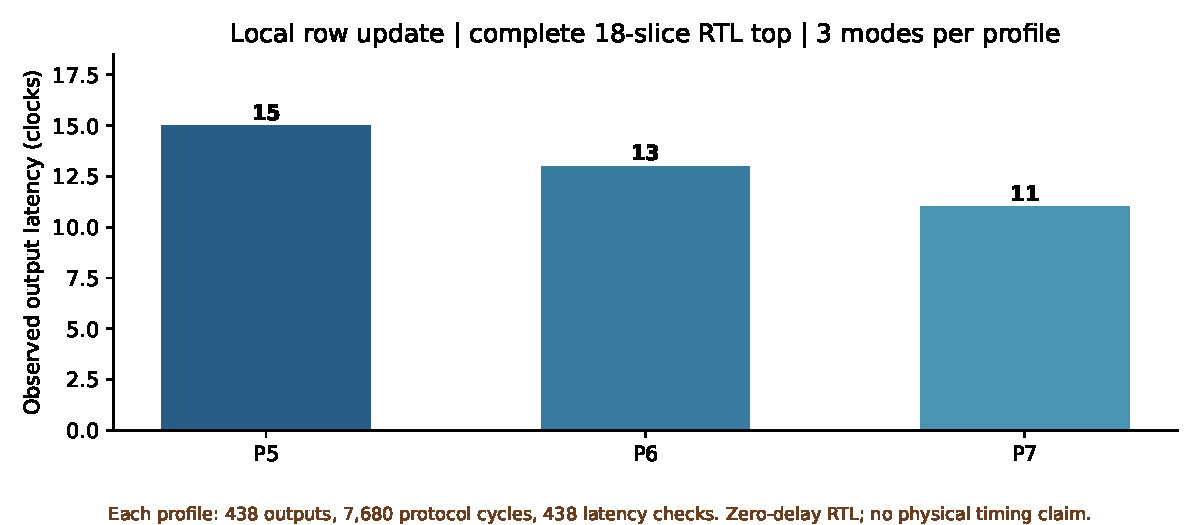
\includegraphics[width=0.84\textwidth]{figures/local_row_profiles.pdf}
\caption{局部行更新候选的实际RTL完整顶层输出延迟。三档结构的输出、周期和延迟检查数均从冻结日志重绘；脚本在作图前核对57项证据文件哈希，见\code{audit_figures/make_local_row_profiles.py}与同名\code{*.sha256.json}。柱高是数字时钟拍数，不能读作纳秒时序。}
\label{fig:local-row-profiles}
\end{figure}

\subsection{如何判定候选可以进入最终版本}
功能门禁要同时覆盖新状态不变量与使用缓存的真实生产链路。
直接驱动 \code{w_rom} 的叶模块保留常量参数关闭缓存的接口；
生产顶层开启缓存，两条路径均有独立标量参考。
定向验证应包含完整最大值行、同址连续替换、clear后重装、拒写、
32\(\times\)128边界、重复与无效ID，以及蓄意损坏一个缓存项后的失败见证。
完整结构顶层还须覆盖18个slice、三种dither模式、配置读回及 epoch 取消。

PPA门禁必须与精简P5采用相同25\,ns约束、器件和工具。
只报源码运算符削减，或只通过缓存关闭分支的回归，都不能算这一候选成功。
即使综合资源下降，仍须实际布局布线检查 setup、hold、pulse width、约束覆盖和DRC，
并对最终完整综合网表执行功能比较。

% Candidate-only evidence; root decides the final insertion point.
\subsection{行和缓存候选的双版本数值证据}
\label{sec:row-cache-evidence}
本节对应候选 RTL 内容摘要 \code{1e3fab94b7b2}\ldots，包含 26 项生产 RTL 文件；父提交为 \code{f028ec5}。
来源为 \code{docs/evidence/20260930/row_cache/}，属于新的本地功能验收，不能移用父提交 CI 的通过结论。
归档中的 Verilator 5.020 与运行时标识为 5.49 的开发版，分别完成相同的五种加载器几何和七种归约器几何。
每个版本的 16,150 个加载事务步与 1,430,848 个归约输入样本按各自单位列示，不相加为覆盖率。
5.020 的附加复验只包括这两项，不能据此声称该工具本地重跑了全部 22 个 bench。

最大装载先把整张表写为 \(W_{\max}=2^{47}-1\)，故每个含 \(U\) 项的物理行应为 \(U W_{\max}\)。
\code{clear_load} 清除完整性位图，保留权重与行和；随后将行 0 的一个旧最大权重替换为 1，
独立期望成为 \mbox{\((U-1)W_{\max}+1\)}。图\ref{fig:row-cache-evidence}分别保留原日志的 \code{row_last} 与 \code{row0} 标签。
制图器以 Python 任意精度整数重新计算，不把超过 \(2^{53}\) 的行和先转为浮点数再判断相等。
全部十个阶段观测在两个版本原始日志中逐条匹配；归档没有单独记录 clear 当拍的数值，因而不额外绘制该时刻。

\begin{figure}[H]\centering
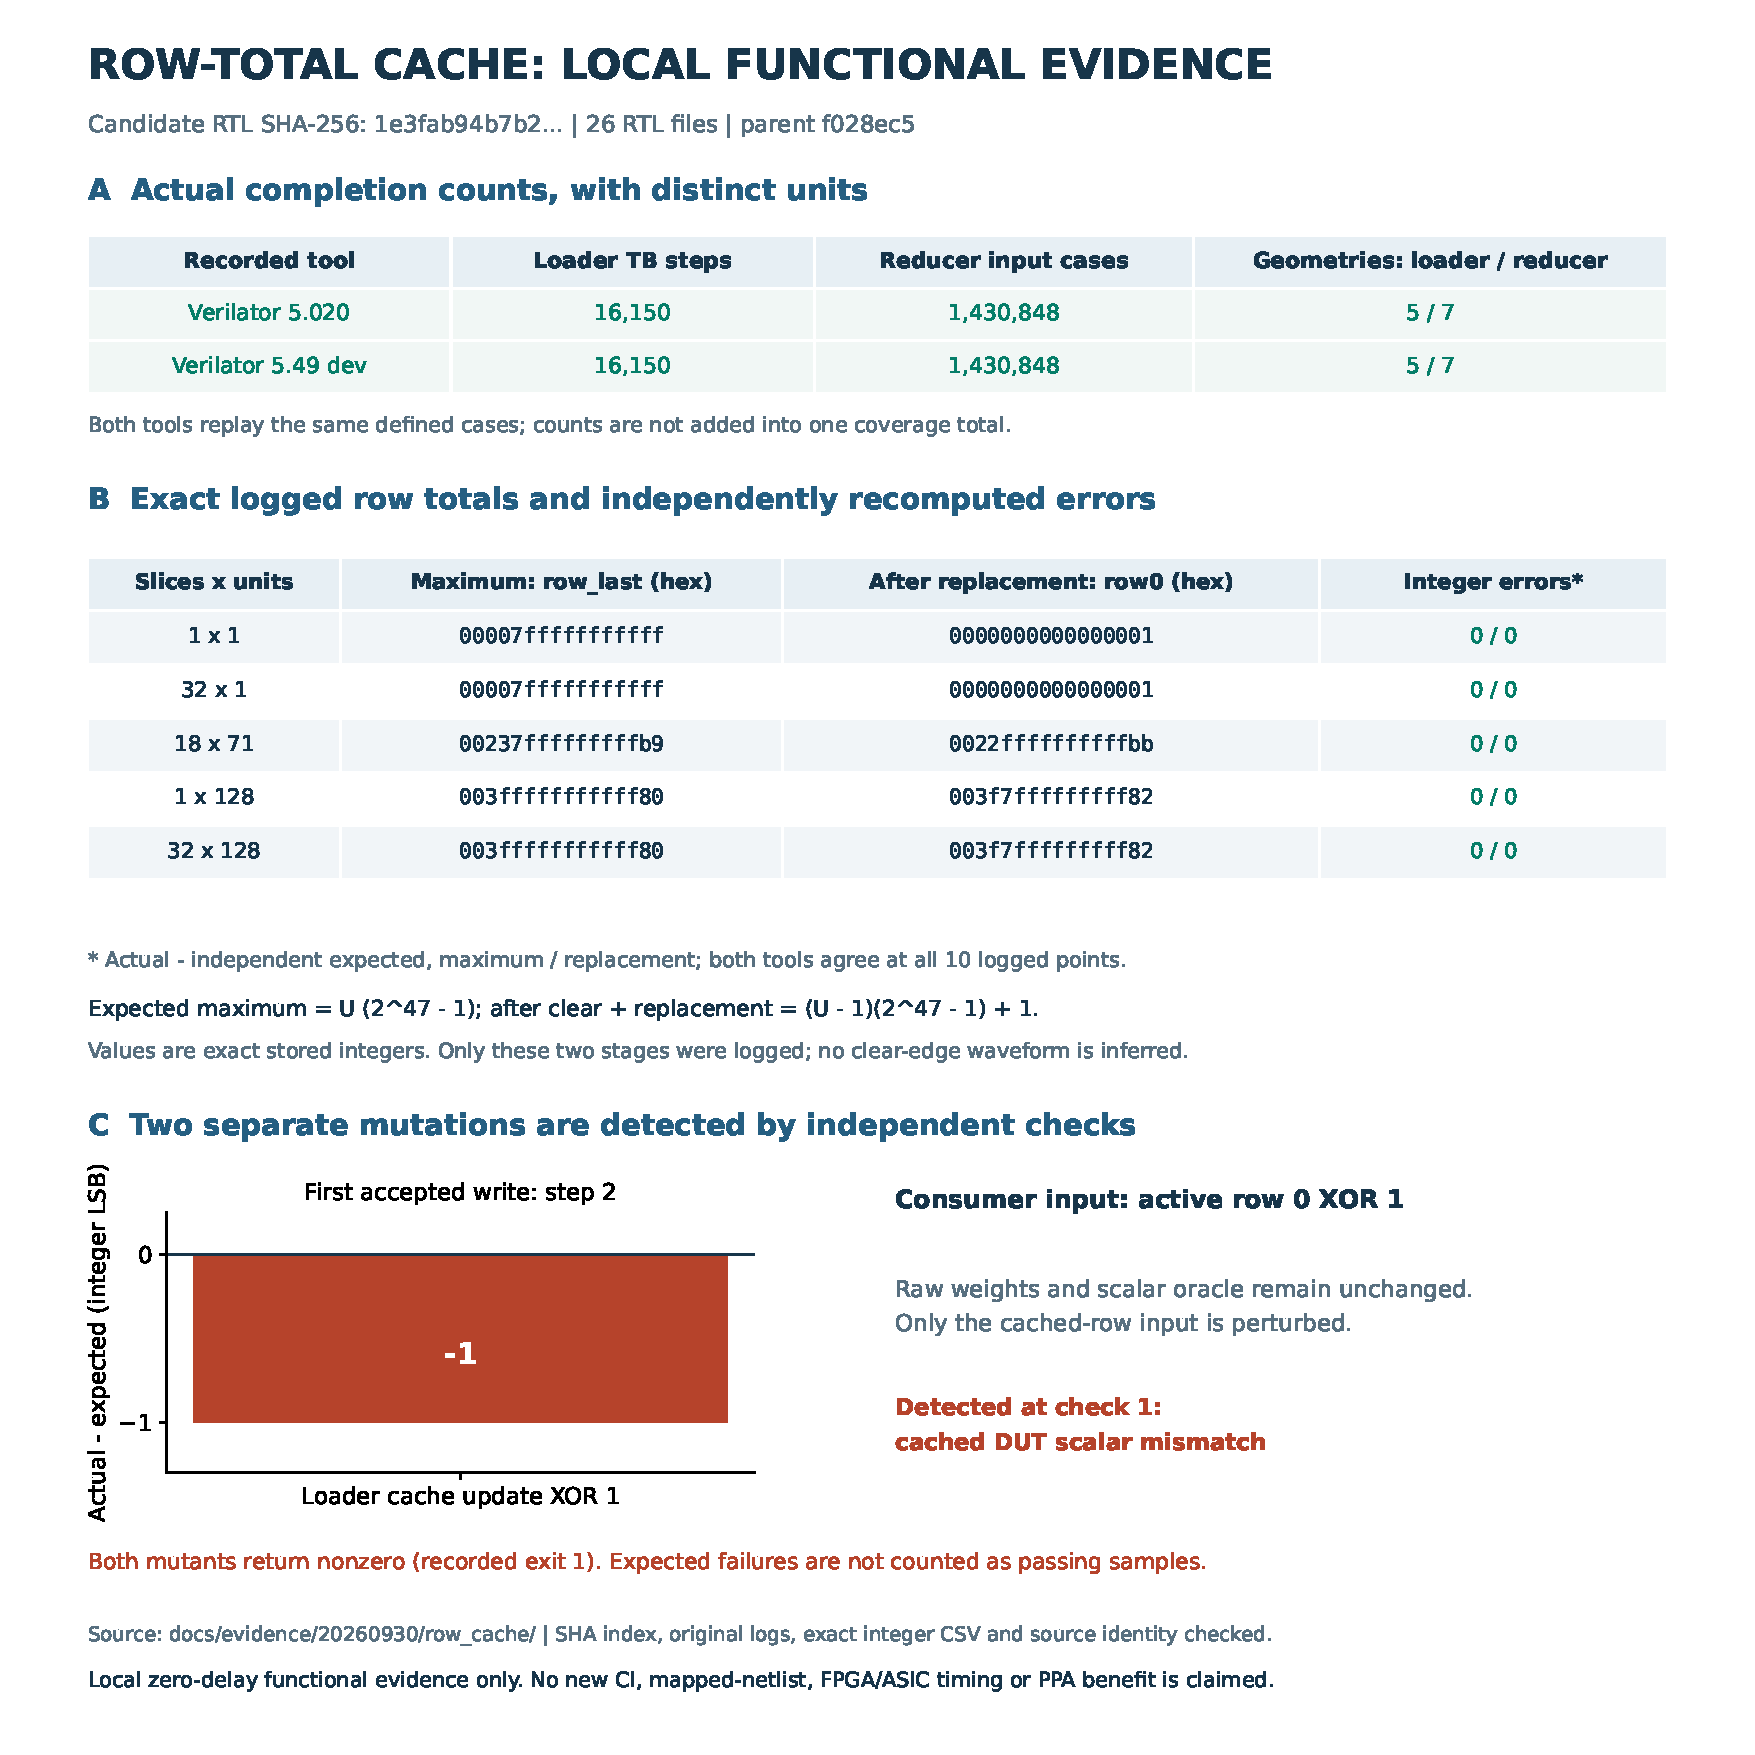
\includegraphics[width=\textwidth]{figures/41_row_cache_evidence.pdf}
\caption{候选行和缓存的真实日志证据。上表为双版本完成计数；中表为五种几何在最大装载和 clear 后替换两个已记录阶段的精确十六进制整数，独立整数公式的误差均为零。下方展示两个分别注入的错误被检出；没有由完成标记推造波形，也没有将功能通过解释为 PPA 收益。}
\label{fig:row-cache-evidence}
\end{figure}

两个负控分别检查生产者和消费者。
第一项只翻转行和写回结果的最低位，在首次接受写的第 2 步出现实际值相对独立期望少 1，加载器检查立即失败。
第二项只翻转活动行 0 的缓存输入最低位，原始权重、未缓存实现、旧公式和 scalar oracle 都不变；
第 1 个比较样本触发 \code{cached DUT scalar mismatch}。
后者排除了“缓存输入被忽略而仍通过普通数值回归”的假阳性；它不是新功能正常输出的样本。

可复现入口为 \code{audit_figures/make_row_cache_evidence.py}，来源清单为 \code{audit_figures/41_source_hashes.json}。
脚本校验归档 SHA、26 项 RTL 摘要、完成计数、十个实测值以及两份负控的失败日志与源文件摘要。
这些结果说明行和维护与消费在所测功能条件下符合独立判据；缓存候选的实际资源、物理建立/保持时序及 ASIC 目标频率仍应由同一候选的后续综合和实现报告单独判定。



\section{P5同约束对照的超时记录}
为了判断行和缓存是否真正带来面积与时序收益，已冻结前代精简版和当前缓存版的源码，
计划在相同\code{xc7vx690tffg1761-2}、Vivado 2018.3、\(P_{\rm STAGES}=5\)、25\,ns请求周期、
同一综合脚本与XDC下逐项比较。前代精简版的第一轮运行在7,200\,s运行时限处被脚本终止，
结束前仍处于时序优化阶段；没有\code{status.txt}、DCP、完整利用率或时序报告。
该轮原始失败记录见\code{docs/evidence/20260930/vivado_compact_p5_timeout/}，
其manifest摘要为\code{ad645b3f5a9304a69636b39737eb74bd0b2595060190cff0ca1b116f409501dd}。
它只说明在记录的机器负载与时限下未完成综合，不能判为WNS不达标，也不能作缓存版的PPA基线。
只有两份完整且通过无驱动检查的报告都取得后，才能填写同约束资源差值。

\subsection{当前缓存版 P5 的有效综合后快照}
当前行和缓存提交的冻结源码另在相同器件、Vivado 2018.3、P5、25\,ns申请周期下完成了一次完整 OOC 综合。
其实际远端运行\code{run.c97c940ad1274c699c40b8c78ff00602}返回\code{SYNTH_COMPLETE}；
原始\code{scp}回传在900\,s上限中断，保留失败manifest后从\emph{同一次远端运行}独立取回全部报告、
续传49,687,597字节DCP，并与远端SHA-256逐字节核对。其完整摘要由下面两行连续拼接：
\par\noindent\code{670d019aaec0efe80e060342ff0dbd74}\quad
\code{8c0029b4c01d6a42e741de32ecb05ff1}。\par
归档\code{docs/evidence/20260930/vivado_cached_p5/}的25个payload文件均通过\code{sha256.json}复验；
恢复过程没有重新综合、替换输入源码或删除传输失败记录。
原始综合日志无\code{Synth 8-3848}无驱动诊断，\code{check_timing}的16类检查全为零，
DRC无错误但有49项警告。这使下面的\emph{综合后}数值可用，但不构成布线或板级时序签核。

\begin{table}[H]\centering\small
\begin{tabular}{lrrl}\toprule
指标&实测值&器件可用值/端点总数&判读\\\midrule
Slice LUT&106,205&433,200&24.52\%\\
触发器&66,520&866,400&7.68\%\\
DSP48E1&20&3,600&0.56\%\\
BRAM tile/锁存器&0/0&1,470/866,400&未推断出BRAM\\
setup WNS/TNS&+10.640\,ns/0&200,389&失效端点0\\
hold WHS/THS&$-0.264$\,ns/$-14,943.110$\,ns&200,389&失效端点60,455\\
pulse WPWS/TPWS&+12.150\,ns/0&66,520&失效端点0\\\bottomrule
\end{tabular}
\caption{冻结的当前缓存版P5完整顶层OOC综合后报告。25\,ns是申请周期；setup通过而hold未通过，因此“全时序满足”和“40\,MHz已实现”都不是本表结论。}
\label{tab:cached-p5-synth}
\end{table}
\begin{figure}[H]\centering
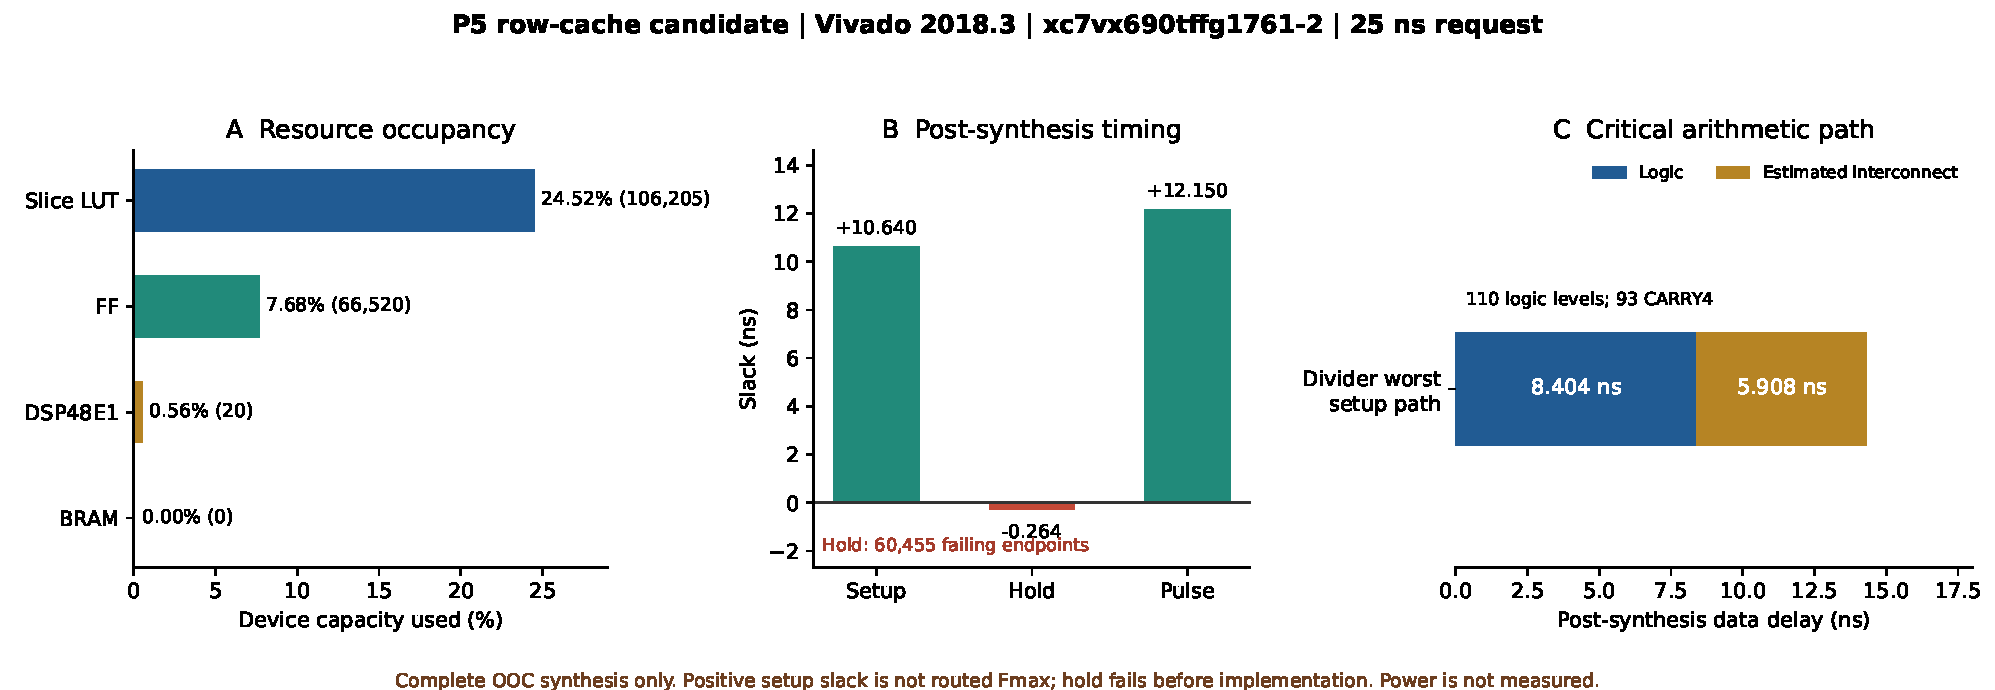
\includegraphics[width=\textwidth]{figures/cached_p5_synthesis.pdf}
\caption{当前缓存版P5的原始\code{utilization.rpt}、\code{timing_summary.rpt}和\code{timing_paths.rpt}重绘：A为器件资源占用，B将setup/hold/pulse分开，C拆出最坏除法路径的逻辑延迟与\emph{综合后估算}互连延迟。图中25\,ns为申请约束，hold负值仍然保留；脚本与来源哈希见\code{audit_figures/make_cached_p5_synth_evidence.py}及同名\code{*.sha256.json}。}
\end{figure}

最坏setup路径仍是\code{u_recon/u_div/rem_reg[0]/C}到\code{u_recon/u_div/q_reg[60]/D}：
估算数据路径14.312\,ns，110级逻辑，含93级CARRY4；该路径没有因行和缓存自动消失。
hold负裕量与未布线、无真实内部时钟缓冲的OOC状态有关，是否能由布局布线消除仍需后述BUFG实跑判定。
这一单独快照与前代P5的超时记录不能构成同约束资源收益；
也不能把此处的P5数值同P7的1.5625\,ns数据归因为缓存效果。
当前P5的\code{power_vectorless.rpt}另给出总功耗0.408\,W，其中动态0.083\,W、静态0.324\,W；
报告标明\code{Simulation Activity File=---}、置信等级Medium，并警告高扇出复位网络的活动假设可能使估算失准。
它不是活动数据标注的实测值；与下节P7的1.580\,W来自不同的周期及结构配置，不能相减作为缓存节能量。

\subsection{完整顶层综合映射后的功能见证}
为检验上述有效P5网表是否只在报告中保留面积数字、却在功能上丢失输入因果，
本轮从同一49,687,597字节DCP导出Vivado 2018.3功能网表，使用XSim直接实例化完整
\code{sar20_digital_core}。测试台仅驱动公开端口，不用\code{force}或读取内部信号；
它配置18个物理单元，逐项读回3,900次配置值，并运行三种确定性输入模式。
第一次尝试因DCP设计名为\code{checkpoint_post_synth}而非预设顶层名，在仿真前停止；
第二次尝试发现Vivado把多维端口拆成58个转义行端口，在\code{xelab}处停止。
修正\emph{测试台连接及导出流程}后的第三次运行才得到\code{FULL\_MAPPED\_FUNCTIONAL\_PASS}；
三次原始记录全部保留，不能将前两次称为功能通过。

最终运行的\code{xsim.log}明示三模式共438个输出行、7,680项协议检查和三次取消。
本地另从CSV逐行复算：每种模式146个有效sample ID，2--158之间各跳过11个，
159为取消；438个\code{code}与测试台独立期望值一致，438个\code{flags}均与期望0一致。
每种模式相邻的145对已接受样本满足
\(\Delta\texttt{clock}=16\Delta\texttt{sample\_id}\)，合计435对。
原始trace、日志及96项payload哈希见
\code{docs/evidence/20260930/vivado_cached_p5_full_mapped/}；
其中trace的SHA-256由下面两行连续拼接：
\par\noindent\code{c40ce4404bbbeae26df514be6484722}\quad
\code{682f936a626c56bd156ada9b5ae8d2073}。\par

\begin{figure}[H]\centering
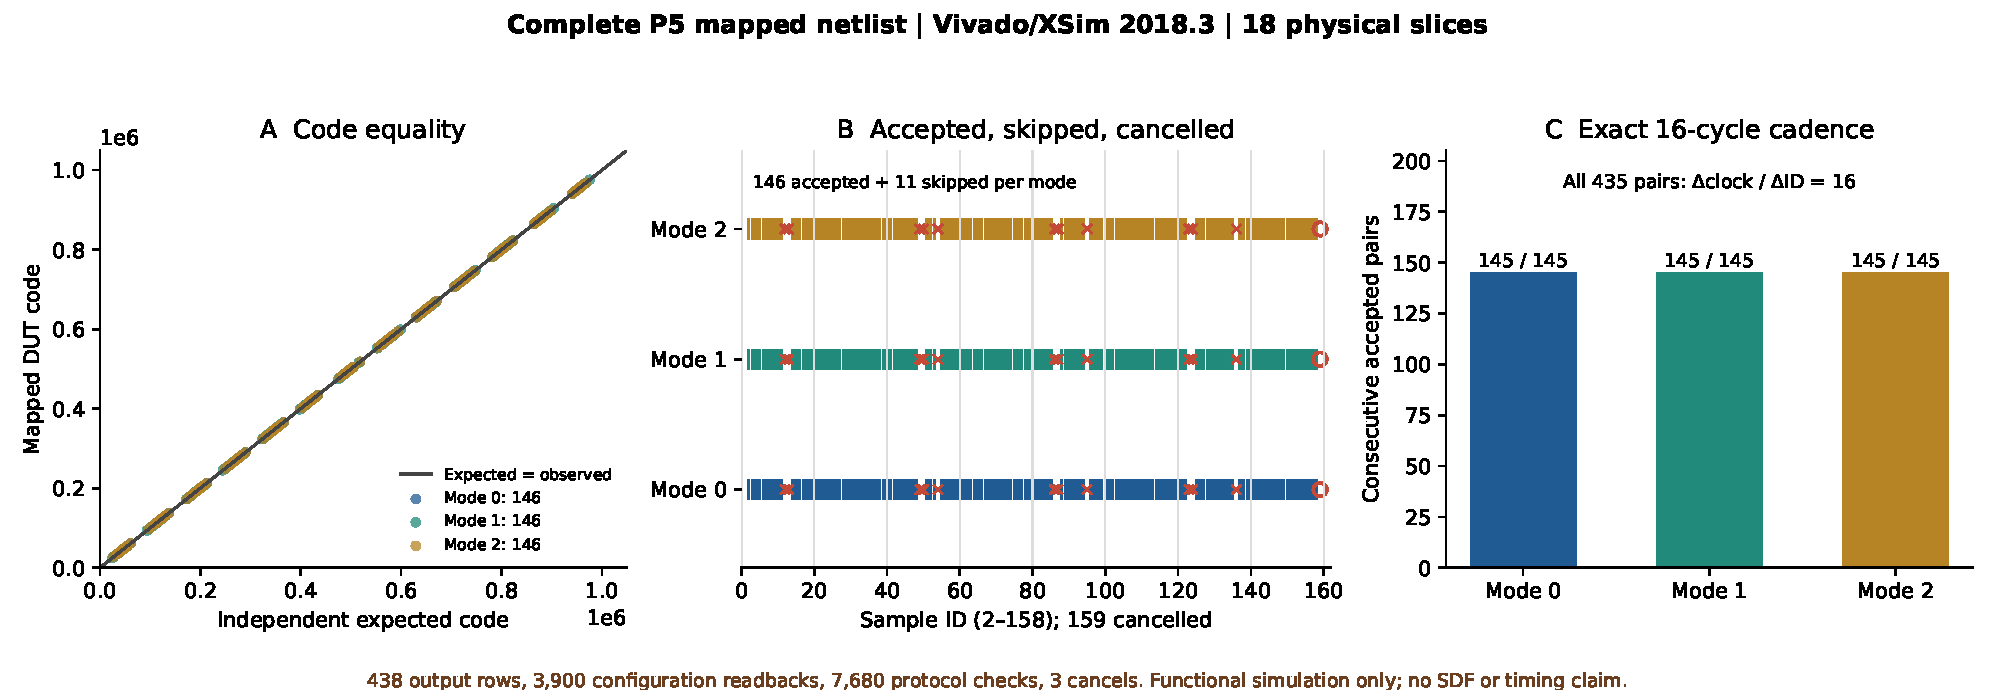
\includegraphics[width=\textwidth]{figures/mapped_p5_full_top.pdf}
\caption{完整P5顶层功能网表的实际XSim CSV：A逐点对照独立期望码，B标出每模式146个有效、11个跳过及取消样本，C检查435对相邻有效输出的16拍/样本ID节拍。原始数据和图件由\code{audit_figures/make_mapped_p5_evidence.py}及同名\code{*.sha256.json}逐项绑定。它不是SDF仿真，也不验证非零flags、内部启动延迟、模拟宏或物理时序。}
\label{fig:full-mapped-p5}
\end{figure}

这组结果把“已完整综合”进一步推进到\emph{选定刺激下的完整顶层映射功能一致}；
P5综合报告的负hold裕量仍然存在。该见证没有SDF反标，没有非零输出flag激励，
也没有检测内部重构启动延迟，因此既不是全面等价证明，也不是40\,MHz的布线结论。

\section{功耗验收不能由LUT数量替代}
前述P7归约/除法候选的原始\code{power_vectorless.rpt}给出下列模型分项。
它对应1.5625\,ns请求周期、尚未布局布线的网表，\code{Simulation Activity File}为空，
报告置信等级为Medium；这些数值是工具估计，不是芯片或FPGA板卡实测功耗。
\begin{center}
\begin{tabular}{lr}\toprule
模型分项&估计功耗/W\\\midrule
Clocks&0.664\\
Slice Logic&0.319\\
Signals&0.260\\
Dynamic合计&1.243\\
Device Static&0.337\\
Total On-Chip&1.580\\\bottomrule
\end{tabular}
\end{center}
Clocks约占该次模型动态功耗的53.4\%，说明只看LUT数量不能覆盖所有功耗来源。
这个比例也不能移用到25\,ns约束、缓存版本或布线后实现；时钟分项中的Used计数不等于独立时钟域数。
系数在运行期保持不变，并不自动证明其所有时钟网络都停止翻转；新增行和状态的开销必须一起计入。

官方\href{https://docs.amd.com/v/u/2018.3-English/ug907-vivado-power-analysis-optimization}{UG907 v2018.3，第33、78页}
说明向量无关估计依赖输入和控制信号的活动假设，FPGA的CE可用于减少无效状态更新；
这不构成对本设计的节能比例保证。本工程下一轮功耗实验应在相同器件、电压、温度、周期和实现阶段下，
分别记录配置装载、稳定16拍事务流及空闲三个工作区间，再导入各自真实活动数据。
应同时交代活动数据的时间窗口、实例匹配、未标注网络和复位占比，不能用装载期或长时间复位的低活动掩盖正常转换功耗。
若评估每样本能耗，应把稳态功耗除以实际通过的样本率，并单列装载能量，避免把不同吞吐的总瓦数直接排序。

时钟使能、操作数保持和专用时钟门控是不同层级的措施。当前RTL保留单一同步时钟，
本轮不以组合门直接改写时钟，也未完成ASIC集成时钟门控单元的映射、测试使能或时钟树验证。
若后续导入该类ASIC单元，必须重新检查门控建立/保持、复位可达性、测试模式和功能等价；
不能把FPGA的CE映射当成ASIC时钟树已经优化。面积、时序和有活动数据的功耗应分别形成证据，再判断整体PPA取舍。

\section{ASIC 目标仍需什么证据}
ASIC 的 640\,MHz 目标需要指定标准单元库、PVT、负载、时钟树、布线寄生和模拟宏接口预算。
FPGA 的 CARRY4、LUT 和 DSP48E1 与 ASIC 单元的延迟结构不同，不能按单一比例换算。
报告给出的除法分段、精确饱和商缩域和系数预聚合方案，是可以继续综合验证的结构候选；
只有在相同目标库下证明功能和约束完整，再取得有效的面积/时序/活动功耗对照，才能宣称 ASIC PPA 优势。

这一限制不妨碍本轮修复具有明确价值：已经排除了被综合器删除功能的实现方式，
使精确整数校准在 RTL 与映射见证中保持一致，并建立不会把无效网表或负时序当成成功的运行门禁。
后续每一个面积和频率数字都能追溯到相应源码、约束和原始报告，而不依赖文档作者的主观判断。
